\documentclass[11pt]{article}

    \usepackage[breakable]{tcolorbox}
    \usepackage{parskip} % Stop auto-indenting (to mimic markdown behaviour)
    
    \usepackage{iftex}
    \ifPDFTeX
    	\usepackage[T1]{fontenc}
    	\usepackage{mathpazo}
    \else
    	\usepackage{fontspec}
    \fi

    % Basic figure setup, for now with no caption control since it's done
    % automatically by Pandoc (which extracts ![](path) syntax from Markdown).
    \usepackage{graphicx}
    % Maintain compatibility with old templates. Remove in nbconvert 6.0
    \let\Oldincludegraphics\includegraphics
    % Ensure that by default, figures have no caption (until we provide a
    % proper Figure object with a Caption API and a way to capture that
    % in the conversion process - todo).
    \usepackage{caption}
    \DeclareCaptionFormat{nocaption}{}
    \captionsetup{format=nocaption,aboveskip=0pt,belowskip=0pt}

    \usepackage{float}
    \floatplacement{figure}{H} % forces figures to be placed at the correct location
    \usepackage{xcolor} % Allow colors to be defined
    \usepackage{enumerate} % Needed for markdown enumerations to work
    \usepackage{geometry} % Used to adjust the document margins
    \usepackage{amsmath} % Equations
    \usepackage{amssymb} % Equations
    \usepackage{textcomp} % defines textquotesingle
    % Hack from http://tex.stackexchange.com/a/47451/13684:
    \AtBeginDocument{%
        \def\PYZsq{\textquotesingle}% Upright quotes in Pygmentized code
    }
    \usepackage{upquote} % Upright quotes for verbatim code
    \usepackage{eurosym} % defines \euro
    \usepackage[mathletters]{ucs} % Extended unicode (utf-8) support
    \usepackage{fancyvrb} % verbatim replacement that allows latex
    \usepackage{grffile} % extends the file name processing of package graphics 
                         % to support a larger range
    \makeatletter % fix for old versions of grffile with XeLaTeX
    \@ifpackagelater{grffile}{2019/11/01}
    {
      % Do nothing on new versions
    }
    {
      \def\Gread@@xetex#1{%
        \IfFileExists{"\Gin@base".bb}%
        {\Gread@eps{\Gin@base.bb}}%
        {\Gread@@xetex@aux#1}%
      }
    }
    \makeatother
    \usepackage[Export]{adjustbox} % Used to constrain images to a maximum size
    \adjustboxset{max size={0.9\linewidth}{0.9\paperheight}}

    % The hyperref package gives us a pdf with properly built
    % internal navigation ('pdf bookmarks' for the table of contents,
    % internal cross-reference links, web links for URLs, etc.)
    \usepackage{hyperref}
    % The default LaTeX title has an obnoxious amount of whitespace. By default,
    % titling removes some of it. It also provides customization options.
    \usepackage{titling}
    \usepackage{longtable} % longtable support required by pandoc >1.10
    \usepackage{booktabs}  % table support for pandoc > 1.12.2
    \usepackage[inline]{enumitem} % IRkernel/repr support (it uses the enumerate* environment)
    \usepackage[normalem]{ulem} % ulem is needed to support strikethroughs (\sout)
                                % normalem makes italics be italics, not underlines
    \usepackage{mathrsfs}
    

    
    % Colors for the hyperref package
    \definecolor{urlcolor}{rgb}{0,.145,.698}
    \definecolor{linkcolor}{rgb}{.71,0.21,0.01}
    \definecolor{citecolor}{rgb}{.12,.54,.11}

    % ANSI colors
    \definecolor{ansi-black}{HTML}{3E424D}
    \definecolor{ansi-black-intense}{HTML}{282C36}
    \definecolor{ansi-red}{HTML}{E75C58}
    \definecolor{ansi-red-intense}{HTML}{B22B31}
    \definecolor{ansi-green}{HTML}{00A250}
    \definecolor{ansi-green-intense}{HTML}{007427}
    \definecolor{ansi-yellow}{HTML}{DDB62B}
    \definecolor{ansi-yellow-intense}{HTML}{B27D12}
    \definecolor{ansi-blue}{HTML}{208FFB}
    \definecolor{ansi-blue-intense}{HTML}{0065CA}
    \definecolor{ansi-magenta}{HTML}{D160C4}
    \definecolor{ansi-magenta-intense}{HTML}{A03196}
    \definecolor{ansi-cyan}{HTML}{60C6C8}
    \definecolor{ansi-cyan-intense}{HTML}{258F8F}
    \definecolor{ansi-white}{HTML}{C5C1B4}
    \definecolor{ansi-white-intense}{HTML}{A1A6B2}
    \definecolor{ansi-default-inverse-fg}{HTML}{FFFFFF}
    \definecolor{ansi-default-inverse-bg}{HTML}{000000}

    % common color for the border for error outputs.
    \definecolor{outerrorbackground}{HTML}{FFDFDF}

    % commands and environments needed by pandoc snippets
    % extracted from the output of `pandoc -s`
    \providecommand{\tightlist}{%
      \setlength{\itemsep}{0pt}\setlength{\parskip}{0pt}}
    \DefineVerbatimEnvironment{Highlighting}{Verbatim}{commandchars=\\\{\}}
    % Add ',fontsize=\small' for more characters per line
    \newenvironment{Shaded}{}{}
    \newcommand{\KeywordTok}[1]{\textcolor[rgb]{0.00,0.44,0.13}{\textbf{{#1}}}}
    \newcommand{\DataTypeTok}[1]{\textcolor[rgb]{0.56,0.13,0.00}{{#1}}}
    \newcommand{\DecValTok}[1]{\textcolor[rgb]{0.25,0.63,0.44}{{#1}}}
    \newcommand{\BaseNTok}[1]{\textcolor[rgb]{0.25,0.63,0.44}{{#1}}}
    \newcommand{\FloatTok}[1]{\textcolor[rgb]{0.25,0.63,0.44}{{#1}}}
    \newcommand{\CharTok}[1]{\textcolor[rgb]{0.25,0.44,0.63}{{#1}}}
    \newcommand{\StringTok}[1]{\textcolor[rgb]{0.25,0.44,0.63}{{#1}}}
    \newcommand{\CommentTok}[1]{\textcolor[rgb]{0.38,0.63,0.69}{\textit{{#1}}}}
    \newcommand{\OtherTok}[1]{\textcolor[rgb]{0.00,0.44,0.13}{{#1}}}
    \newcommand{\AlertTok}[1]{\textcolor[rgb]{1.00,0.00,0.00}{\textbf{{#1}}}}
    \newcommand{\FunctionTok}[1]{\textcolor[rgb]{0.02,0.16,0.49}{{#1}}}
    \newcommand{\RegionMarkerTok}[1]{{#1}}
    \newcommand{\ErrorTok}[1]{\textcolor[rgb]{1.00,0.00,0.00}{\textbf{{#1}}}}
    \newcommand{\NormalTok}[1]{{#1}}
    
    % Additional commands for more recent versions of Pandoc
    \newcommand{\ConstantTok}[1]{\textcolor[rgb]{0.53,0.00,0.00}{{#1}}}
    \newcommand{\SpecialCharTok}[1]{\textcolor[rgb]{0.25,0.44,0.63}{{#1}}}
    \newcommand{\VerbatimStringTok}[1]{\textcolor[rgb]{0.25,0.44,0.63}{{#1}}}
    \newcommand{\SpecialStringTok}[1]{\textcolor[rgb]{0.73,0.40,0.53}{{#1}}}
    \newcommand{\ImportTok}[1]{{#1}}
    \newcommand{\DocumentationTok}[1]{\textcolor[rgb]{0.73,0.13,0.13}{\textit{{#1}}}}
    \newcommand{\AnnotationTok}[1]{\textcolor[rgb]{0.38,0.63,0.69}{\textbf{\textit{{#1}}}}}
    \newcommand{\CommentVarTok}[1]{\textcolor[rgb]{0.38,0.63,0.69}{\textbf{\textit{{#1}}}}}
    \newcommand{\VariableTok}[1]{\textcolor[rgb]{0.10,0.09,0.49}{{#1}}}
    \newcommand{\ControlFlowTok}[1]{\textcolor[rgb]{0.00,0.44,0.13}{\textbf{{#1}}}}
    \newcommand{\OperatorTok}[1]{\textcolor[rgb]{0.40,0.40,0.40}{{#1}}}
    \newcommand{\BuiltInTok}[1]{{#1}}
    \newcommand{\ExtensionTok}[1]{{#1}}
    \newcommand{\PreprocessorTok}[1]{\textcolor[rgb]{0.74,0.48,0.00}{{#1}}}
    \newcommand{\AttributeTok}[1]{\textcolor[rgb]{0.49,0.56,0.16}{{#1}}}
    \newcommand{\InformationTok}[1]{\textcolor[rgb]{0.38,0.63,0.69}{\textbf{\textit{{#1}}}}}
    \newcommand{\WarningTok}[1]{\textcolor[rgb]{0.38,0.63,0.69}{\textbf{\textit{{#1}}}}}
    
    
    % Define a nice break command that doesn't care if a line doesn't already
    % exist.
    \def\br{\hspace*{\fill} \\* }
    % Math Jax compatibility definitions
    \def\gt{>}
    \def\lt{<}
    \let\Oldtex\TeX
    \let\Oldlatex\LaTeX
    \renewcommand{\TeX}{\textrm{\Oldtex}}
    \renewcommand{\LaTeX}{\textrm{\Oldlatex}}
    % Document parameters
    % Document title
    \title{Ejercicios Programación Lineal}

    
\usepackage{mdframed}


\newenvironment{problem}[2][Problema]
    { \begin{mdframed}[backgroundcolor=gray!20] \textbf{#1 #2} \\}
    {  \end{mdframed}}

% Define solution environment
\newenvironment{solution}
    {\textit{Solución}}
    {}
    

    \usepackage{fancyhdr} % Headers and footers
    \pagestyle{fancy} % All pages have headers and footers
    \fancyhead{}\renewcommand{\headrulewidth}{0pt} % Blank out the default header
    \fancyfoot[L]{} % Custom footer text
    \fancyfoot[C]{} % Custom footer text
    \fancyfoot[R]{\thepage} % Custom footer text
    \newcommand{\note}[1]{\marginpar{\scriptsize \textcolor{red}{#1}}} % Enables comments in red on margin
    
    
    
    
% Pygments definitions
\makeatletter
\def\PY@reset{\let\PY@it=\relax \let\PY@bf=\relax%
    \let\PY@ul=\relax \let\PY@tc=\relax%
    \let\PY@bc=\relax \let\PY@ff=\relax}
\def\PY@tok#1{\csname PY@tok@#1\endcsname}
\def\PY@toks#1+{\ifx\relax#1\empty\else%
    \PY@tok{#1}\expandafter\PY@toks\fi}
\def\PY@do#1{\PY@bc{\PY@tc{\PY@ul{%
    \PY@it{\PY@bf{\PY@ff{#1}}}}}}}
\def\PY#1#2{\PY@reset\PY@toks#1+\relax+\PY@do{#2}}

\expandafter\def\csname PY@tok@w\endcsname{\def\PY@tc##1{\textcolor[rgb]{0.73,0.73,0.73}{##1}}}
\expandafter\def\csname PY@tok@c\endcsname{\let\PY@it=\textit\def\PY@tc##1{\textcolor[rgb]{0.25,0.50,0.50}{##1}}}
\expandafter\def\csname PY@tok@cp\endcsname{\def\PY@tc##1{\textcolor[rgb]{0.74,0.48,0.00}{##1}}}
\expandafter\def\csname PY@tok@k\endcsname{\let\PY@bf=\textbf\def\PY@tc##1{\textcolor[rgb]{0.00,0.50,0.00}{##1}}}
\expandafter\def\csname PY@tok@kp\endcsname{\def\PY@tc##1{\textcolor[rgb]{0.00,0.50,0.00}{##1}}}
\expandafter\def\csname PY@tok@kt\endcsname{\def\PY@tc##1{\textcolor[rgb]{0.69,0.00,0.25}{##1}}}
\expandafter\def\csname PY@tok@o\endcsname{\def\PY@tc##1{\textcolor[rgb]{0.40,0.40,0.40}{##1}}}
\expandafter\def\csname PY@tok@ow\endcsname{\let\PY@bf=\textbf\def\PY@tc##1{\textcolor[rgb]{0.67,0.13,1.00}{##1}}}
\expandafter\def\csname PY@tok@nb\endcsname{\def\PY@tc##1{\textcolor[rgb]{0.00,0.50,0.00}{##1}}}
\expandafter\def\csname PY@tok@nf\endcsname{\def\PY@tc##1{\textcolor[rgb]{0.00,0.00,1.00}{##1}}}
\expandafter\def\csname PY@tok@nc\endcsname{\let\PY@bf=\textbf\def\PY@tc##1{\textcolor[rgb]{0.00,0.00,1.00}{##1}}}
\expandafter\def\csname PY@tok@nn\endcsname{\let\PY@bf=\textbf\def\PY@tc##1{\textcolor[rgb]{0.00,0.00,1.00}{##1}}}
\expandafter\def\csname PY@tok@ne\endcsname{\let\PY@bf=\textbf\def\PY@tc##1{\textcolor[rgb]{0.82,0.25,0.23}{##1}}}
\expandafter\def\csname PY@tok@nv\endcsname{\def\PY@tc##1{\textcolor[rgb]{0.10,0.09,0.49}{##1}}}
\expandafter\def\csname PY@tok@no\endcsname{\def\PY@tc##1{\textcolor[rgb]{0.53,0.00,0.00}{##1}}}
\expandafter\def\csname PY@tok@nl\endcsname{\def\PY@tc##1{\textcolor[rgb]{0.63,0.63,0.00}{##1}}}
\expandafter\def\csname PY@tok@ni\endcsname{\let\PY@bf=\textbf\def\PY@tc##1{\textcolor[rgb]{0.60,0.60,0.60}{##1}}}
\expandafter\def\csname PY@tok@na\endcsname{\def\PY@tc##1{\textcolor[rgb]{0.49,0.56,0.16}{##1}}}
\expandafter\def\csname PY@tok@nt\endcsname{\let\PY@bf=\textbf\def\PY@tc##1{\textcolor[rgb]{0.00,0.50,0.00}{##1}}}
\expandafter\def\csname PY@tok@nd\endcsname{\def\PY@tc##1{\textcolor[rgb]{0.67,0.13,1.00}{##1}}}
\expandafter\def\csname PY@tok@s\endcsname{\def\PY@tc##1{\textcolor[rgb]{0.73,0.13,0.13}{##1}}}
\expandafter\def\csname PY@tok@sd\endcsname{\let\PY@it=\textit\def\PY@tc##1{\textcolor[rgb]{0.73,0.13,0.13}{##1}}}
\expandafter\def\csname PY@tok@si\endcsname{\let\PY@bf=\textbf\def\PY@tc##1{\textcolor[rgb]{0.73,0.40,0.53}{##1}}}
\expandafter\def\csname PY@tok@se\endcsname{\let\PY@bf=\textbf\def\PY@tc##1{\textcolor[rgb]{0.73,0.40,0.13}{##1}}}
\expandafter\def\csname PY@tok@sr\endcsname{\def\PY@tc##1{\textcolor[rgb]{0.73,0.40,0.53}{##1}}}
\expandafter\def\csname PY@tok@ss\endcsname{\def\PY@tc##1{\textcolor[rgb]{0.10,0.09,0.49}{##1}}}
\expandafter\def\csname PY@tok@sx\endcsname{\def\PY@tc##1{\textcolor[rgb]{0.00,0.50,0.00}{##1}}}
\expandafter\def\csname PY@tok@m\endcsname{\def\PY@tc##1{\textcolor[rgb]{0.40,0.40,0.40}{##1}}}
\expandafter\def\csname PY@tok@gh\endcsname{\let\PY@bf=\textbf\def\PY@tc##1{\textcolor[rgb]{0.00,0.00,0.50}{##1}}}
\expandafter\def\csname PY@tok@gu\endcsname{\let\PY@bf=\textbf\def\PY@tc##1{\textcolor[rgb]{0.50,0.00,0.50}{##1}}}
\expandafter\def\csname PY@tok@gd\endcsname{\def\PY@tc##1{\textcolor[rgb]{0.63,0.00,0.00}{##1}}}
\expandafter\def\csname PY@tok@gi\endcsname{\def\PY@tc##1{\textcolor[rgb]{0.00,0.63,0.00}{##1}}}
\expandafter\def\csname PY@tok@gr\endcsname{\def\PY@tc##1{\textcolor[rgb]{1.00,0.00,0.00}{##1}}}
\expandafter\def\csname PY@tok@ge\endcsname{\let\PY@it=\textit}
\expandafter\def\csname PY@tok@gs\endcsname{\let\PY@bf=\textbf}
\expandafter\def\csname PY@tok@gp\endcsname{\let\PY@bf=\textbf\def\PY@tc##1{\textcolor[rgb]{0.00,0.00,0.50}{##1}}}
\expandafter\def\csname PY@tok@go\endcsname{\def\PY@tc##1{\textcolor[rgb]{0.53,0.53,0.53}{##1}}}
\expandafter\def\csname PY@tok@gt\endcsname{\def\PY@tc##1{\textcolor[rgb]{0.00,0.27,0.87}{##1}}}
\expandafter\def\csname PY@tok@err\endcsname{\def\PY@bc##1{\setlength{\fboxsep}{0pt}\fcolorbox[rgb]{1.00,0.00,0.00}{1,1,1}{\strut ##1}}}
\expandafter\def\csname PY@tok@kc\endcsname{\let\PY@bf=\textbf\def\PY@tc##1{\textcolor[rgb]{0.00,0.50,0.00}{##1}}}
\expandafter\def\csname PY@tok@kd\endcsname{\let\PY@bf=\textbf\def\PY@tc##1{\textcolor[rgb]{0.00,0.50,0.00}{##1}}}
\expandafter\def\csname PY@tok@kn\endcsname{\let\PY@bf=\textbf\def\PY@tc##1{\textcolor[rgb]{0.00,0.50,0.00}{##1}}}
\expandafter\def\csname PY@tok@kr\endcsname{\let\PY@bf=\textbf\def\PY@tc##1{\textcolor[rgb]{0.00,0.50,0.00}{##1}}}
\expandafter\def\csname PY@tok@bp\endcsname{\def\PY@tc##1{\textcolor[rgb]{0.00,0.50,0.00}{##1}}}
\expandafter\def\csname PY@tok@fm\endcsname{\def\PY@tc##1{\textcolor[rgb]{0.00,0.00,1.00}{##1}}}
\expandafter\def\csname PY@tok@vc\endcsname{\def\PY@tc##1{\textcolor[rgb]{0.10,0.09,0.49}{##1}}}
\expandafter\def\csname PY@tok@vg\endcsname{\def\PY@tc##1{\textcolor[rgb]{0.10,0.09,0.49}{##1}}}
\expandafter\def\csname PY@tok@vi\endcsname{\def\PY@tc##1{\textcolor[rgb]{0.10,0.09,0.49}{##1}}}
\expandafter\def\csname PY@tok@vm\endcsname{\def\PY@tc##1{\textcolor[rgb]{0.10,0.09,0.49}{##1}}}
\expandafter\def\csname PY@tok@sa\endcsname{\def\PY@tc##1{\textcolor[rgb]{0.73,0.13,0.13}{##1}}}
\expandafter\def\csname PY@tok@sb\endcsname{\def\PY@tc##1{\textcolor[rgb]{0.73,0.13,0.13}{##1}}}
\expandafter\def\csname PY@tok@sc\endcsname{\def\PY@tc##1{\textcolor[rgb]{0.73,0.13,0.13}{##1}}}
\expandafter\def\csname PY@tok@dl\endcsname{\def\PY@tc##1{\textcolor[rgb]{0.73,0.13,0.13}{##1}}}
\expandafter\def\csname PY@tok@s2\endcsname{\def\PY@tc##1{\textcolor[rgb]{0.73,0.13,0.13}{##1}}}
\expandafter\def\csname PY@tok@sh\endcsname{\def\PY@tc##1{\textcolor[rgb]{0.73,0.13,0.13}{##1}}}
\expandafter\def\csname PY@tok@s1\endcsname{\def\PY@tc##1{\textcolor[rgb]{0.73,0.13,0.13}{##1}}}
\expandafter\def\csname PY@tok@mb\endcsname{\def\PY@tc##1{\textcolor[rgb]{0.40,0.40,0.40}{##1}}}
\expandafter\def\csname PY@tok@mf\endcsname{\def\PY@tc##1{\textcolor[rgb]{0.40,0.40,0.40}{##1}}}
\expandafter\def\csname PY@tok@mh\endcsname{\def\PY@tc##1{\textcolor[rgb]{0.40,0.40,0.40}{##1}}}
\expandafter\def\csname PY@tok@mi\endcsname{\def\PY@tc##1{\textcolor[rgb]{0.40,0.40,0.40}{##1}}}
\expandafter\def\csname PY@tok@il\endcsname{\def\PY@tc##1{\textcolor[rgb]{0.40,0.40,0.40}{##1}}}
\expandafter\def\csname PY@tok@mo\endcsname{\def\PY@tc##1{\textcolor[rgb]{0.40,0.40,0.40}{##1}}}
\expandafter\def\csname PY@tok@ch\endcsname{\let\PY@it=\textit\def\PY@tc##1{\textcolor[rgb]{0.25,0.50,0.50}{##1}}}
\expandafter\def\csname PY@tok@cm\endcsname{\let\PY@it=\textit\def\PY@tc##1{\textcolor[rgb]{0.25,0.50,0.50}{##1}}}
\expandafter\def\csname PY@tok@cpf\endcsname{\let\PY@it=\textit\def\PY@tc##1{\textcolor[rgb]{0.25,0.50,0.50}{##1}}}
\expandafter\def\csname PY@tok@c1\endcsname{\let\PY@it=\textit\def\PY@tc##1{\textcolor[rgb]{0.25,0.50,0.50}{##1}}}
\expandafter\def\csname PY@tok@cs\endcsname{\let\PY@it=\textit\def\PY@tc##1{\textcolor[rgb]{0.25,0.50,0.50}{##1}}}

\def\PYZbs{\char`\\}
\def\PYZus{\char`\_}
\def\PYZob{\char`\{}
\def\PYZcb{\char`\}}
\def\PYZca{\char`\^}
\def\PYZam{\char`\&}
\def\PYZlt{\char`\<}
\def\PYZgt{\char`\>}
\def\PYZsh{\char`\#}
\def\PYZpc{\char`\%}
\def\PYZdl{\char`\$}
\def\PYZhy{\char`\-}
\def\PYZsq{\char`\'}
\def\PYZdq{\char`\"}
\def\PYZti{\char`\~}
% for compatibility with earlier versions
\def\PYZat{@}
\def\PYZlb{[}
\def\PYZrb{]}
\makeatother


    % For linebreaks inside Verbatim environment from package fancyvrb. 
    \makeatletter
        \newbox\Wrappedcontinuationbox 
        \newbox\Wrappedvisiblespacebox 
        \newcommand*\Wrappedvisiblespace {\textcolor{red}{\textvisiblespace}} 
        \newcommand*\Wrappedcontinuationsymbol {\textcolor{red}{\llap{\tiny$\m@th\hookrightarrow$}}} 
        \newcommand*\Wrappedcontinuationindent {3ex } 
        \newcommand*\Wrappedafterbreak {\kern\Wrappedcontinuationindent\copy\Wrappedcontinuationbox} 
        % Take advantage of the already applied Pygments mark-up to insert 
        % potential linebreaks for TeX processing. 
        %        {, <, #, %, $, ' and ": go to next line. 
        %        _, }, ^, &, >, - and ~: stay at end of broken line. 
        % Use of \textquotesingle for straight quote. 
        \newcommand*\Wrappedbreaksatspecials {% 
            \def\PYGZus{\discretionary{\char`\_}{\Wrappedafterbreak}{\char`\_}}% 
            \def\PYGZob{\discretionary{}{\Wrappedafterbreak\char`\{}{\char`\{}}% 
            \def\PYGZcb{\discretionary{\char`\}}{\Wrappedafterbreak}{\char`\}}}% 
            \def\PYGZca{\discretionary{\char`\^}{\Wrappedafterbreak}{\char`\^}}% 
            \def\PYGZam{\discretionary{\char`\&}{\Wrappedafterbreak}{\char`\&}}% 
            \def\PYGZlt{\discretionary{}{\Wrappedafterbreak\char`\<}{\char`\<}}% 
            \def\PYGZgt{\discretionary{\char`\>}{\Wrappedafterbreak}{\char`\>}}% 
            \def\PYGZsh{\discretionary{}{\Wrappedafterbreak\char`\#}{\char`\#}}% 
            \def\PYGZpc{\discretionary{}{\Wrappedafterbreak\char`\%}{\char`\%}}% 
            \def\PYGZdl{\discretionary{}{\Wrappedafterbreak\char`\$}{\char`\$}}% 
            \def\PYGZhy{\discretionary{\char`\-}{\Wrappedafterbreak}{\char`\-}}% 
            \def\PYGZsq{\discretionary{}{\Wrappedafterbreak\textquotesingle}{\textquotesingle}}% 
            \def\PYGZdq{\discretionary{}{\Wrappedafterbreak\char`\"}{\char`\"}}% 
            \def\PYGZti{\discretionary{\char`\~}{\Wrappedafterbreak}{\char`\~}}% 
        } 
        % Some characters . , ; ? ! / are not pygmentized. 
        % This macro makes them "active" and they will insert potential linebreaks 
        \newcommand*\Wrappedbreaksatpunct {% 
            \lccode`\~`\.\lowercase{\def~}{\discretionary{\hbox{\char`\.}}{\Wrappedafterbreak}{\hbox{\char`\.}}}% 
            \lccode`\~`\,\lowercase{\def~}{\discretionary{\hbox{\char`\,}}{\Wrappedafterbreak}{\hbox{\char`\,}}}% 
            \lccode`\~`\;\lowercase{\def~}{\discretionary{\hbox{\char`\;}}{\Wrappedafterbreak}{\hbox{\char`\;}}}% 
            \lccode`\~`\:\lowercase{\def~}{\discretionary{\hbox{\char`\:}}{\Wrappedafterbreak}{\hbox{\char`\:}}}% 
            \lccode`\~`\?\lowercase{\def~}{\discretionary{\hbox{\char`\?}}{\Wrappedafterbreak}{\hbox{\char`\?}}}% 
            \lccode`\~`\!\lowercase{\def~}{\discretionary{\hbox{\char`\!}}{\Wrappedafterbreak}{\hbox{\char`\!}}}% 
            \lccode`\~`\/\lowercase{\def~}{\discretionary{\hbox{\char`\/}}{\Wrappedafterbreak}{\hbox{\char`\/}}}% 
            \catcode`\.\active
            \catcode`\,\active 
            \catcode`\;\active
            \catcode`\:\active
            \catcode`\?\active
            \catcode`\!\active
            \catcode`\/\active 
            \lccode`\~`\~ 	
        }
    \makeatother

    \let\OriginalVerbatim=\Verbatim
    \makeatletter
    \renewcommand{\Verbatim}[1][1]{%
        %\parskip\z@skip
        \sbox\Wrappedcontinuationbox {\Wrappedcontinuationsymbol}%
        \sbox\Wrappedvisiblespacebox {\FV@SetupFont\Wrappedvisiblespace}%
        \def\FancyVerbFormatLine ##1{\hsize\linewidth
            \vtop{\raggedright\hyphenpenalty\z@\exhyphenpenalty\z@
                \doublehyphendemerits\z@\finalhyphendemerits\z@
                \strut ##1\strut}%
        }%
        % If the linebreak is at a space, the latter will be displayed as visible
        % space at end of first line, and a continuation symbol starts next line.
        % Stretch/shrink are however usually zero for typewriter font.
        \def\FV@Space {%
            \nobreak\hskip\z@ plus\fontdimen3\font minus\fontdimen4\font
            \discretionary{\copy\Wrappedvisiblespacebox}{\Wrappedafterbreak}
            {\kern\fontdimen2\font}%
        }%
        
        % Allow breaks at special characters using \PYG... macros.
        \Wrappedbreaksatspecials
        % Breaks at punctuation characters . , ; ? ! and / need catcode=\active 	
        \OriginalVerbatim[#1,codes*=\Wrappedbreaksatpunct]%
    }
    \makeatother

    % Exact colors from NB
    \definecolor{incolor}{HTML}{303F9F}
    \definecolor{outcolor}{HTML}{D84315}
    \definecolor{cellborder}{HTML}{CFCFCF}
    \definecolor{cellbackground}{HTML}{F7F7F7}
    
    % prompt
    \makeatletter
    \newcommand{\boxspacing}{\kern\kvtcb@left@rule\kern\kvtcb@boxsep}
    \makeatother
    \newcommand{\prompt}[4]{
        {\ttfamily\llap{{\color{#2}[#3]:\hspace{3pt}#4}}\vspace{-\baselineskip}}
    }
    
    \pagestyle{fancy}

    
    % Prevent overflowing lines due to hard-to-break entities
    \sloppy 
    % Setup hyperref package
    \hypersetup{
      breaklinks=true,  % so long urls are correctly broken across lines
      colorlinks=true,
      urlcolor=urlcolor,
      linkcolor=linkcolor,
      citecolor=citecolor,
      }
    % Slightly bigger margins than the latex defaults
    
    \geometry{verbose,tmargin=1in,bmargin=1in,lmargin=1in,rmargin=1in}
    
    

\begin{document}
    
    %-------------------------------
%	TITLE SECTION
%-------------------------------

\fancyhead[C]{}
\hrule \medskip % Upper rule
\begin{minipage}{0.295\textwidth}
\raggedright
\footnotesize
Francisco Javier Sáez Maldonado \hfill\\
José Antonio Álvarez Ocete \hfill\\
\end{minipage}
\begin{minipage}{0.4\textwidth}
\centering
\large
Ejercicios Programación Lineal\\
\normalsize
Optimización\\
\end{minipage}
\begin{minipage}{0.295\textwidth}
\raggedleft
\today\hfill\\
\end{minipage}
\medskip\hrule
\bigskip

%-------------------------------
%	CONTENTS
%-------------------------------

    
\begin{problem}{3.c}
Resolver geométricamente el siguiente problema de programación lineal:
\begin{align*}
\min \quad z  = 2x_1 + 5x_2\\
\text{subject to} \\
x_1 + x_2 & \geq 4 \\
x_1 & \geq 2\\
x_1,x_2 & \geq 0
\end{align*}
    \end{problem}

Dibujamos la solución en la Figura \ref{fig:ej3c}.

\begin{figure}
    \centering  
    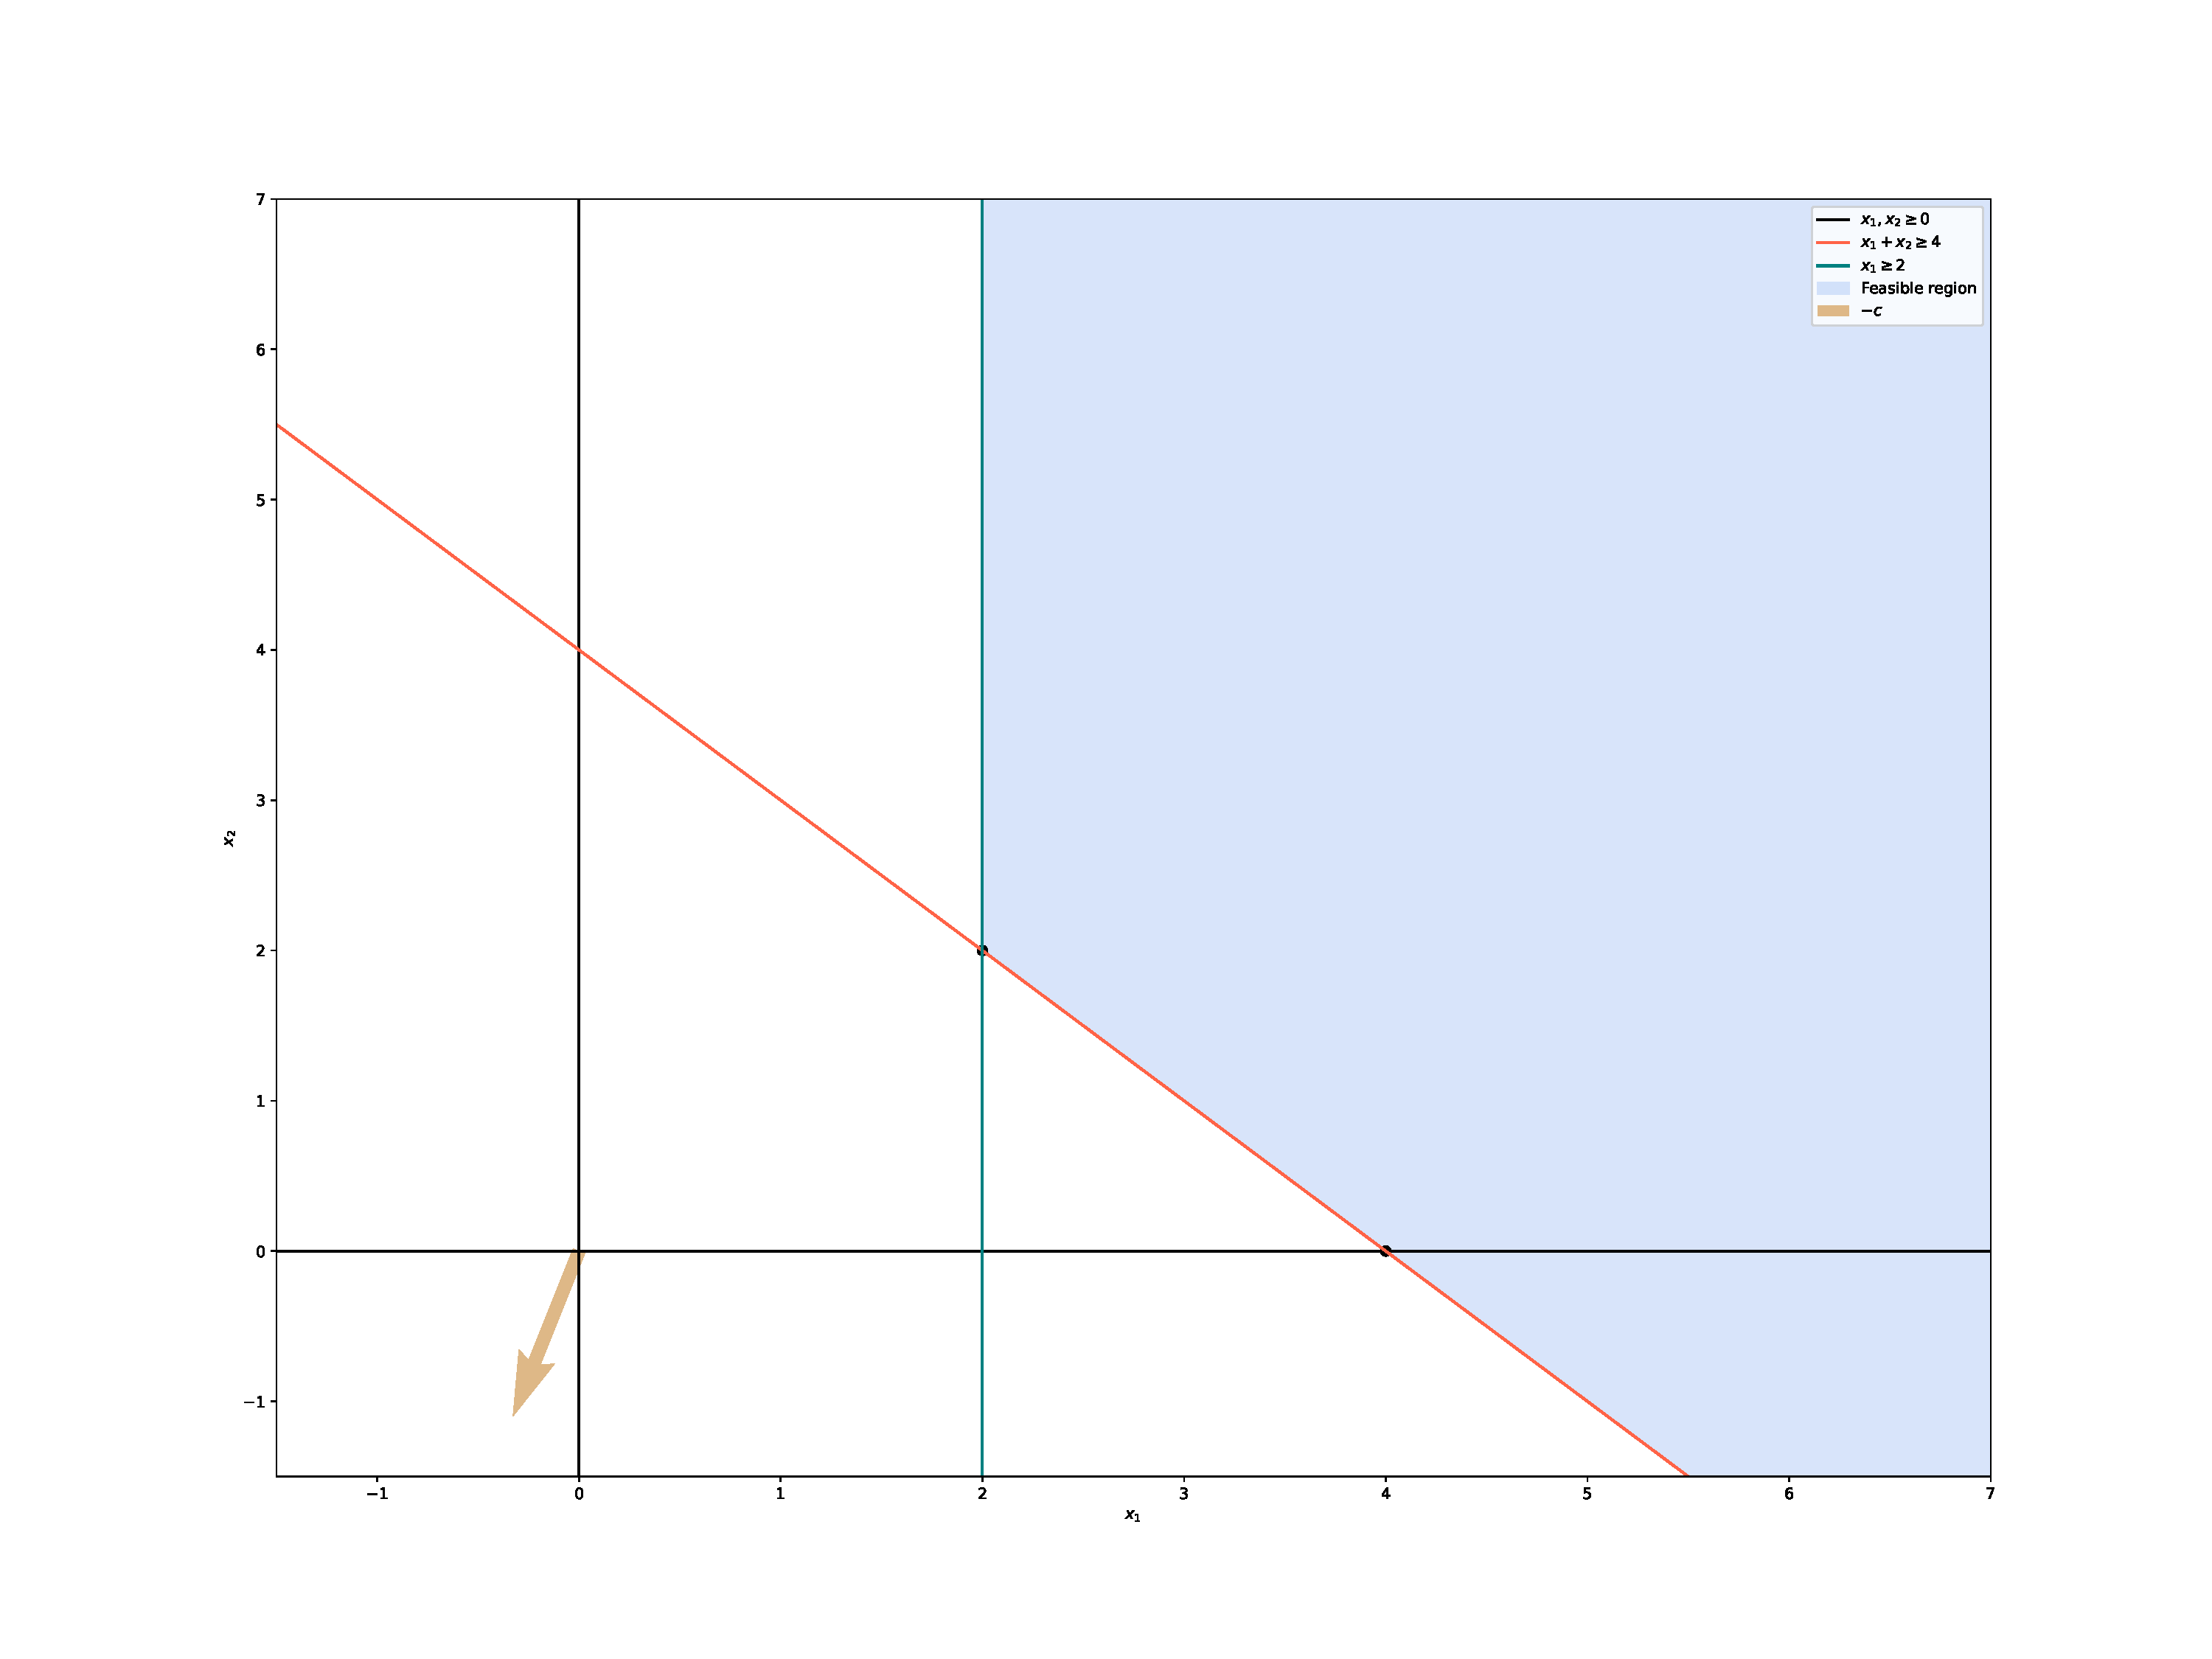
\includegraphics[scale=0.8]{Ej3c}
    \caption{Región factible y puntos solución del problema 3.c)}
    \label{fig:ej3c}
\end{figure}

Tenemos una región factible no acotada, pero tenemos una solución óptima y única, pues si tomamos la dirección que nos da $-c$, llegamos al punto $(4,0)$, descartando el otro punto extremo $(2,2)$ ya que según la dirección de $-c$, la función objetivo decrece más hacia abajo que hacia la izquierda. Por tanto, podemos decir que el mínimo es $f(4,0) = 8$.\\

    
    \begin{problem}{9.c}

    Resolver el siguiente problema de P.L. mediante el algoritmo simplex y el mismo algoritmo en formato de tabla.

      \begin{align*}
        \max z = 2x_{1} + 5x_{2} \\
        \text{subject to} \\
        x_{1} + x_{2} & \leq 4\\
        x_{1} \geq 2\\
        x_{1},x_{2} \geq 0
    \end{align*}

    Primero, expresamos el problema añadiendo variables de holgura:

    \begin{align*}
        \max z = 2x_{1} + 5x_{2} \\
        \text{subject to} \\
        x_{1} + x_{2} - x_{3} & = 4\\
        x_{1} - x_{4} =  2\\
        x_{1},x_{2},x_{3},x_{4} \geq 0
    \end{align*}

    Vamos a resolverlo ahora por los dos métodos mencionados.\\

    \textbf{Método Algebraico.}\\

    Tenemos los siguientes elementos:
    \[
    A = \begin{pmatrix} 1 & 1 & -1 & 0 \\ 1 & 0 & 0 & -1\end{pmatrix}, \quad b = \begin{pmatrix} 4 \\ 2\end{pmatrix}, \quad c = \begin{pmatrix} 2 & 5\end{pmatrix}{T}   
    \]

    Ahora, vamos a escribir \(A = \begin{pmatrix} B & N \end{pmatrix}\). Seleccionamos como \(B\) la matriz
    \[
    B = \begin{pmatrix} 1 & 1 \\ 1 & 0 \end{pmatrix} \implies B^{-1} = \begin{pmatrix}    0 & 1 \\ 1 & -1 \end{pmatrix}
    \]
    Ahora, tenemos que 
    \[
    x_B = B^{-1}b =      \begin{pmatrix}    0 & 1 \\ 1 & -1 \end{pmatrix} \begin{pmatrix} 4 \\ 2\end{pmatrix} = \begin{pmatrix} 2 \\ 2 \end{pmatrix},
    \]
    y que, el valor de la función objetivo es:
    \[
    z = c_B B^{-1}b = \begin{pmatrix} 2 & 5\end{pmatrix} \begin{pmatrix}    0 & 1 \\ 1 & -1 \end{pmatrix} \begin{pmatrix} 4 \\ 2\end{pmatrix}   = \begin{pmatrix} 2 & 5\end{pmatrix}  \begin{pmatrix} 2 \\ 2 \end{pmatrix} = 14.
    \]
    Tenemos que calcular para todas las variables no básicas los valores
    \[
    z_j - c_j = c_B B^{-1}a_j - c_j.
    \]
    Los valores obtenidos son:
    \[
    z_3 - c_3 =     \begin{pmatrix} 2 & 5\end{pmatrix} \begin{pmatrix}    0 & 1 \\ 1 & -1 \end{pmatrix} \begin{pmatrix} -1 \\ 0 \end{pmatrix} - 0 = -5
    \]
    \[
    z_4 - c_4 =     \begin{pmatrix} 2 & 5\end{pmatrix} \begin{pmatrix}    0 & 1 \\ 1 & -1 \end{pmatrix} \begin{pmatrix} 0 \\ -1 \end{pmatrix} - 0 = 3
    \]

    Ahora, tomamos el máximo de estos, que es \(z_4 - c_4 = 3\). Como no se cumple que sea menor que \(0\), la variable \(x_4\) entra en la base.


    \end{problem}
        
    
        \begin{problem}{10}
          Dado el siguiente PPL:
          \begin{align*}
            P: \ \min \ x_{1} - 2x_{2}\\
            \text{subject to} \\
            3x_{1} + 4x_{2} = 12 \\
            2x_{1} - x_{2} \leq 12\\
            x_{1},x_{2} \geq 0
          \end{align*}
          \begin{enumerate}
            \item Plantear el PPL en forma estándar
            \item Resolver geométricamente. Expresar: (a) la región factible, (b) el vector de costes, (c) la función objetivo, (d)  los puntos extremos y sus coordenadas, (e) el punto o puntos solución y el valor objetivo óptimo en el/los mismo/s.
                  \item Resuélvelo aplicando el algoritmo simples algebraico a la SBF dada por la submatriz básica \(B=(a_{2} \ a_{3}\). Debes indicar la solución y el valor objetivo óptimo, justificando por qué lo son.
                  \end{enumerate}
            \end{problem}

            \begin{enumerate}
                \item Para que este problema esté en forma estándar, todas las restricciones del problema deben ser de igualdad. Es por ello que debemos eliminar la restricción de desigualdad de este caso añadiendo una variable de holgura. El problema quedaría del siguiente modo:

                \begin{align*}
                    P: \ \min \ x_{1} - 2x_{2}\\
                    \text{subject to} \\
                    3x_{1} + 4x_{2} = 12 \\
                    2x_{1} - x_{2} + x_{3} = 12\\
                    x_{1},x_{2},x_{3} \geq 0
                  \end{align*}

                  \item Vamos ahora a resolverlo geométricamente. Primero, identificamos los elementos:
                  \begin{enumerate}
                    \item Dibujamos la región factible (que en este caso está sobre la recta definida por una de las restricciones) en la Figura \ref{fig:ej10}.
                    \begin{figure}
                        
                        \centering  
                        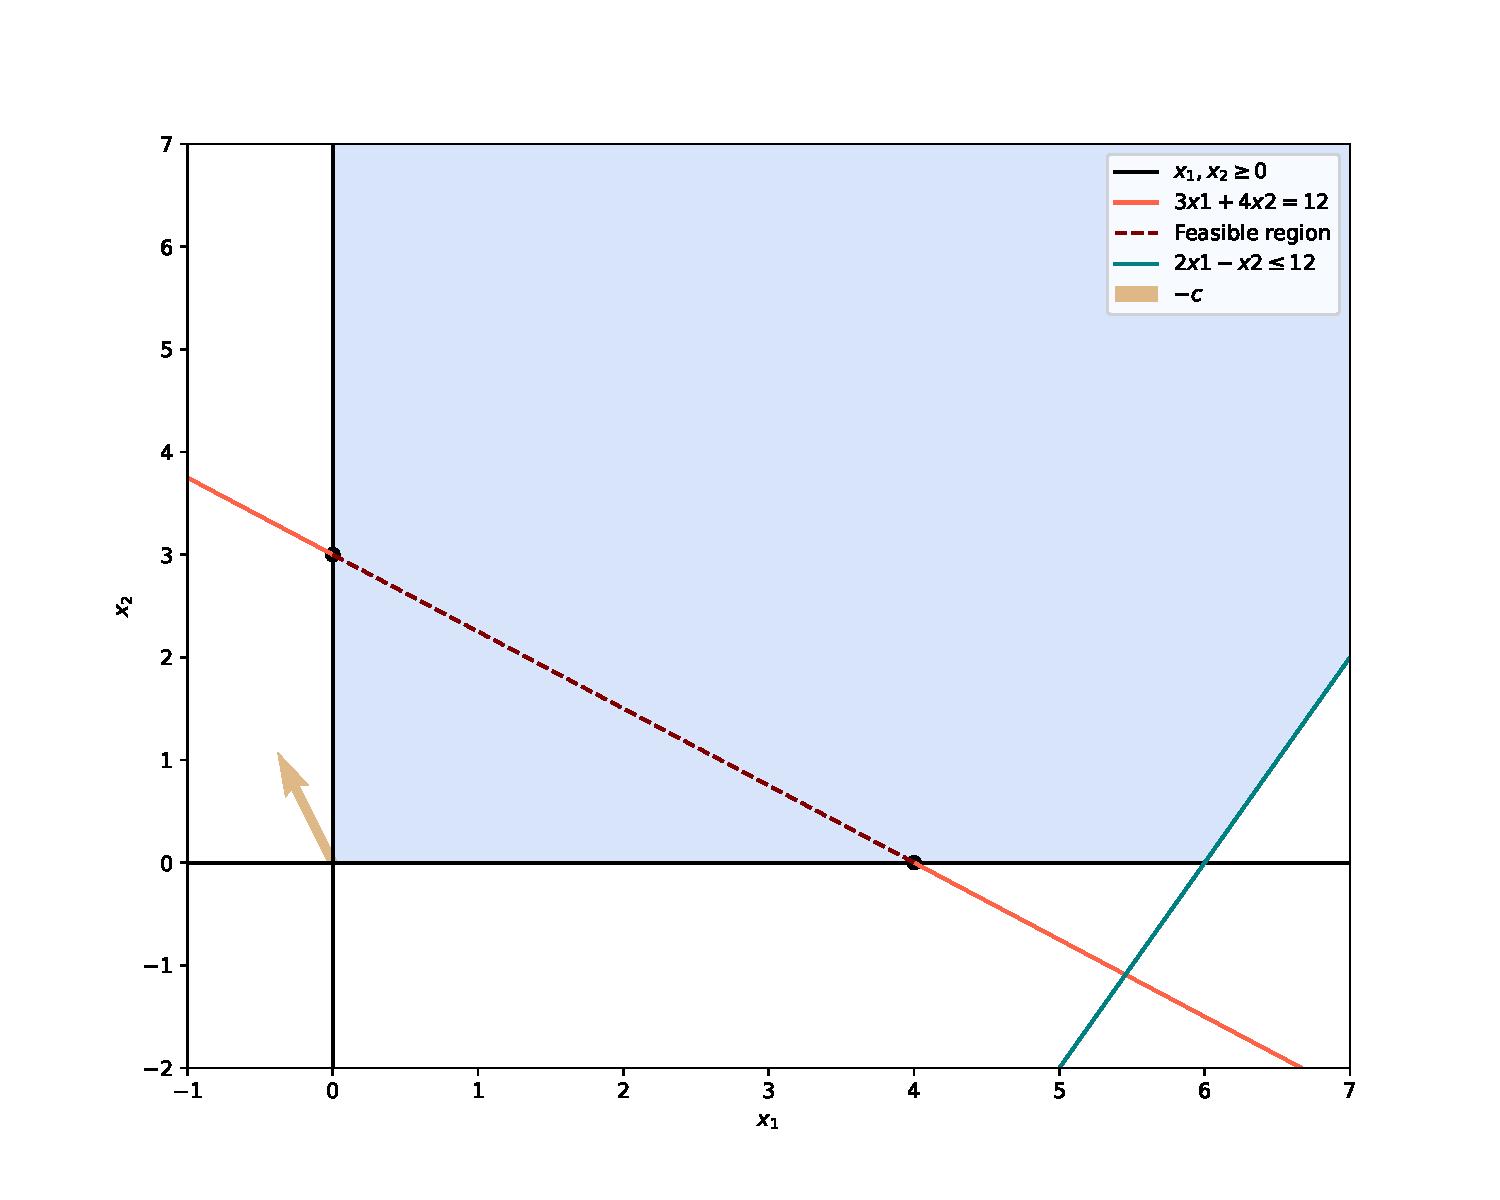
\includegraphics[scale=0.8]{Ej10}
                        \caption{Región factible y puntos solución del problema.}
                        \label{fig:ej10}
                    \end{figure}
                  \item El vector de costes es el vector \(c\) tal que la función a minimizar es \(c^T x\), por lo que en este caso \(c = (1,-2)\).
                  \item La función objetivo es esta función a minimizar, en este caso
                  \[
                  f(x_1,x_2) = c^T(x_1,x_2) = x_1 - 2 x_2.  
                  \]
                  \item Los puntos extremos son los que hemos dibujado en la Figura \ref{Fig:ej10}, que son los puntos donde se cortan las restricciones. En este caso, son el \((0,3)\) y el \(4,0)\)
                  \item Si utilizamos la dirección del vector \(-c\), dibujada también en la figura,  vemos que la solución óptima se da en el punto \((0,3)\) y tiene valor \(f(0,3) = -6\).
                  
                \end{enumerate}

                \item Vamos ahora a resolverlo aplicando el algoritmo simplex algebraico. Consideramos la SBF inicial dada por la submatriz básica \(B = (a_2 \ \ a_3)\) (queda así hecho el \textbf{Paso 1}).\\ 
                
                \textbf{Paso 2.}\\
                Primero, vemos que nuestra matriz \(A\) es :
                \[
                A = \begin{pmatrix} 3 & 4 & 0 \\  2 & -1 & 1 \end{pmatrix}        
                \]
                Por lo que, en este caso, 
                \[
                B = \begin{pmatrix} 4 & 0 \\ -1 & 1\end{pmatrix}, \implies B^{-1} = \begin{pmatrix} \frac{1}{4} & 0 \\ \frac{1}{4} & 1\end{pmatrix}.
                \]
                Y tenemos también que \(c_B = (-2,0)\). Conociendo el vector \(b = (12 \ 12)^T\), podemos calcular el valor de las variables básicas:
                \[
                x_B = B^{-1} b = \begin{pmatrix} \frac{1}{4} & 0 \\ \frac{1}{4} & 1\end{pmatrix} \begin{pmatrix} 12 \\ 12 \end{pmatrix}  = \begin{pmatrix} 3 & 15\end{pmatrix}
                \]
                Calculamos entonces el valor de la función objetivo:
                \[
                z = c_B B^{-1} b = (-2,0)  \begin{pmatrix} \frac{1}{4} & 0 \\ \frac{1}{4} & 1\end{pmatrix} \begin{pmatrix} 12 \\ 12\end{pmatrix} = -6
                \]
                \textbf{Paso 3.}\\
                A continuación, solo tenemos una variable no básica \(a_1\), debemos calcular \(z_j - c_j\) para esta variable no básica. Tenemos que:
                \[
                z_j - c_j = c_b B^{-1}a_j - c_j =  \begin{pmatrix} \frac{1}{4} & 0 \\ \frac{1}{4} & 1\end{pmatrix}\begin{pmatrix} 3 \\ 2 \end{pmatrix} - 2 = -\frac{3}{2} - 1 = -\frac{5}{2} < 0
                \]
                Ahora, como \(z_1 - c_1 \leq 0\), se verifica el \textbf{criterio de optimalidad simplex} (que es que todas las variables no básicas verifiquen esta desigualdad) y por tanto hemos terminado el algoritmo, por lo que nuestra \textbf{SBF actual es óptima}. \\
                Para finalizar, sabemos que como \(x_1\) finalizó como variable no básica, su valor es \(0\), y el valor de \(x_2\) lo encontramos previamente cuando calculamos \(x_B = B^-1 b\), y vimos que era \(x_2 = 3\). Es por ello que nuestra solución óptima de este problema está en el punto \((x_1,x_2) = (0,3)\) y tiene el valor calculado previamente \(z = c_B B^{-1} b = -6 \).\\
            \end{enumerate}

\begin{problem}{11}
	Resolver por el método de las dos fases el PPL del ejercicio anterior.
\end{problem}

\emph{Ejercicio realizado por:} José Antonio Álvarez Ocete

El objetivo de la primera fase será obtener una SBF inicial. Para ello buscamos que aparezca en la parte superior de la tabla una matriz identidad. La variable de holgura \(x_3\) nos proporciona la segunda columna de dicha matriz. Para obtener la primera añadimos una variable artificial adicional, \(x_4\). Obtenemos el siguiente problema de minimización:

\[
\begin{align*}
	P: \ \min \ z = x_4\\
	\text{subject to} \\
	3x_{1} + 4x_{2} & = 12 \\
	2x_{1} - x_{2} + x_3 & = 12\\
	x_{1}, x_{2}, x_3, x_4 & \geq 0
\end{align*}
\]

La matriz $A$ tendrá la siguiente expresión:

\[
A = (a_1 \ a_2 \ a_3 \ a_4) =
\begin{pmatrix}
	3 & 4 & 0 & 1\\
	2 & -1 & 1 & 0
\end{pmatrix}.
\]

A continuación mostramos la tabla correspondiente a este problema, partiendo de la SBF inicial dada por $B=(a_4 \ a_3)$, con $B^{-1}=I$. Además de la fila inicial con los valores de la fase I, añadimos una fila con los valores de la fase II para ir computándolos directamente. Así cuando cambiémos de fase bastará con eliminar la fila correspondiente a la fase I y las columnas correspondientes a las variables artificiales (únciamente \(x_4\) en nuestro caso):

\begin{table}[h!]
	\centering
	\begin{tabular}{c|c|cccc|c}
		& z & $x_1$ & $x_2$ & $x_3$ & $x_4$ & LD \\
		\hline
		I & 1 & 0 & 0 & 0 & -1 & 0\\
		II & 1 & -1 & 2 & 0 & 0 & 0\\
		\hline
		$x_4$ & 0 & 3 & 4 & 0 & 1 & 12\\
		$x_3$ & 0 & 2 & -1 & 1 & 0 & 12
	\end{tabular}
\end{table}

En primer lgiar, hacemos ceros en las variables básicas de la primera fila. Para ello, sumamos la fila correspondiente a $x_4$ la priemra fila:

\begin{table}[h!]
	\centering
	\begin{tabular}{c|c|cccc|c}
		& z & $x_1$ & $x_2$ & $x_3$ & $x_4$ & LD \\
		\hline
		I & 1 & 3 & 4 & 0 & 0 & 12 \\
		II & 1 & -1 & 2 & 0 & 0 & 0 \\
		\hline
		$x_4$ & 0 & 3 & 4 & 0 & 1 & 12\\
		$x_3$ & 0 & 2 & -1 & 1 & 0 & 12
	\end{tabular}
\end{table}

Puesto que el elemento \(4\) es máximo en la primera fila, la variable \(x_2\) entrará en la base. Para decidir qué variable sale de la base tomaríamos el mínimo entre los cocientes de la columna LD y la correspondiente a la variable que entra en la base, \(x_2\), sin incluir los valores no positivos. Por lo tanto, la variable que sale en la base es \(x_4\). Obtenemos:

\begin{table}[h!]
	\centering
	\begin{tabular}{c|c|cccc|c}
		& z & $x_1$ & $x_2$ & $x_3$ & $x_4$ & LD \\
		\hline
		I & 1 & 0 & 0 & 0 & -1 & 0\\
		II & 1 & -5/2 & 0 & 0 & -1/2 & -6\\
		\hline
		$x_2$ & 0 & 3/4 & 1 & 0 & 1/4 & 3\\
		$x_3$ & 0 & 11/4 & 0 & 1 & 1/4 & 15
	\end{tabular}
\end{table}

Como no quedan elementos positivos en la primera fila, hemos concluido la fase I. A continuación revisamos si las variables artificales valen \(0\). Como la variable \(x_4\) no está en la base, toma valor nulo y podemos eliminarla de la tabla para proseguir con la fase II con la SBF inicial encontrada $(x_1, x_2)=(0, 3)$, asociada a la matriz básica $B=(a_2 \ a_3)$:

\begin{table}[h!]
	\centering
	\begin{tabular}{c|c|ccc|c}
		& z & $x_1$ & $x_2$ & $x_3$ & $z$\\
		II & 1 & -5/2 & 0 & 0 & -6\\
		\hline
		$x_2$ & 0 & 3/4 & 1 & 0 & 3\\
		$x_3$ & 0 & 11/4 & 0 & 1 & 15
	\end{tabular}
\end{table}

De nuevo, hemos de hacer operaciones para que queden valores positivos en la primera fila. Sin embargo, ya que no quedan valores positivos en dicha fila podemos concluir que hemos terminado de ejecutar el algorimto. La solución óptima será $(x_1, x_2)=(0, 3)$ ya que al no ser \(x_1\) una variable básica toma valor nulo. Dicha solución tiene valor óptimo de la función de coste $z=-6$. Esto coincide con la solución obtenida por el método algebraico utilizado en el problema anterior, como cabría esperar.
    
\end{document}
